\documentclass[a4paper,10pt]{article}
\usepackage[utf8]{inputenc}
\usepackage[english]{babel}
\usepackage{graphicx}
\usepackage{amsmath}

%opening
\title{Network Simulation with ns/2: report}
\author{Maarten Tegelaers \and Thomas Vochten}

\begin{document}

\maketitle

\begin{abstract}
This report describes the use of the ns/2 network event simulator to simulate the behaviour of simple network topologies.
Two topology situations are considered. For the first situation, the focus lies on an FTP application competing for bandwith
with a CBR application. In the second situation, we investigate the evolution of the congestion window size during the
execution of the TCP algorithm in detail; an FTP application is running continuously while a web user on the same LAN as
the FTP application generates short intense bursts of traffic. We also compare congestion window size behaviour between
the Tahoe implementation of TCP and the Reno implementation of TCP.
\end{abstract}

\section{Exercise 1: Bandwith restrictions on KotNet}

\section{Exercise 2: Tahoe and Reno versus bursty web traffic}
\begin{enumerate}
 \item \textbf{Investigate the throughput of the main FTP application. Can you indicate the effects the
 individual bursts of web traffic have on its total throughput? Why do these ffects not immediately
 become visible when each burst starts (i.e. at 5, 10 , or resp. 15 seconds)?} \\
 
 Figure \ref{fig:ex2throughput} shows the throughput of the main FTP application. We can see that the throughput rises
 rapidly at the start before hitting the bandwidth limit within the first 700 milliseconds. Thereafter, it remains at $1.25$
 megabytes/s. When the first burst begins at 5 seconds, we see a drop to 800 kilobytes/s as the first TCP connection for the web user
 starts, but the throughput can still climb to one megabytes/s. It is only after 700 milliseconds that the throughput
 decreases dramatically. When the burst starts, new connections between the web user and the web server are opened within
 about 0.05 milliseconds. These connections first go through the slow start phase of TCP, which means it takes some time
 before each connection attains a throughput that could affect existing connections. Soon, the 10 megabytes/s bandwidth
 limit cannot support high throughputs for each active connection, which means the main FTP connection experiences packet loss. This triggers
 congestion avoidance for the main FTP application and it sets its congestion window to 1 packet, after which it
 must go through slow start again. \\
 
 After about 8 seconds, the main FTP application has to contend with increasingly fewer connections from the web user,
 which allows the throughput to climb steadily. A new burst starts at 10 seconds, and this time the effects manifest
 themselves after 300 milliseconds. This is again explained by connections being opened one after another and
 each connection gradually increasing its throughput. \\
 
 Right before the third burst, the FTP application cuts its throughput because of congestion. The throughput is allowed
 to climb until 15.7 seconds, when the new burst first has an impact. From 17 seconds on, more and more web connections
 finish their work, allowing the FTP application to steadily increase its throughput to the highest allowed bandwidth
 across the network.
 
 \begin{figure}[h]
 \label{fig:ex2throughput}
  \centering
    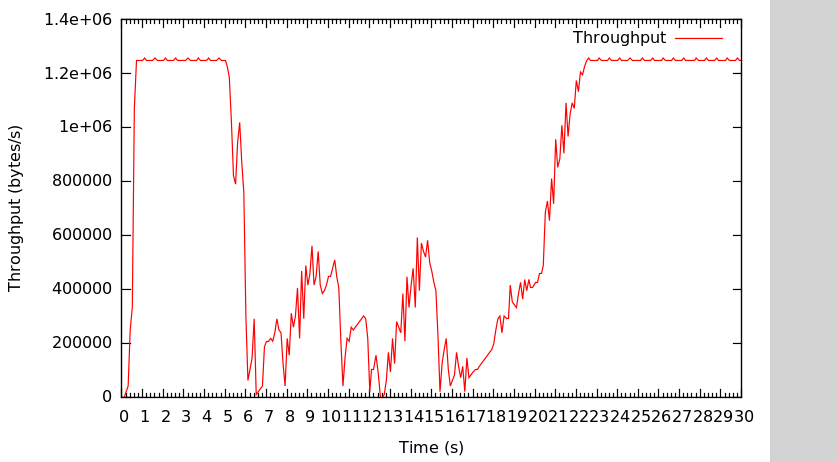
\includegraphics[scale=0.5]{ex2throughput.png}
  \caption{The throughput of the continuously running FTP application. Ticks are drawn every 200 milliseconds.}
 \end{figure}
 
 \item \textbf{Plot the congestion window size and
 slow start thresholds in another graph. Can you identify
 the different phases of the TCP algorithm? When is the
 slow start threshold recalculated and how?} \\
 
 Figure \ref{fig:ex2congestionwindow} shows the congestion window sizes and the slow start thresholds for the main
 FTP application. To start off, the threshold is set to 80 packets and the congestion window size to 1 packet. Each time
 the sender receives an acknowledgement, the congestion window is set to $min(2 \cdot window size, threshold)$.
 This is the slow start phase. Once the threshold has been reached, the window size increases by one each round-trip time.
 This is the additive increase phase. At about 5.76 seconds, the FTP application experiences packet loss, which causes
 the window size to drop to one packet. The slow start threshold is set to $max(2, \frac{threshold}{2})$, which in
 this case is 40. After that, the slow start phase begins again.
 
 \begin{figure}[h]
 \label{fig:ex2congestionwindow}
  \centering
    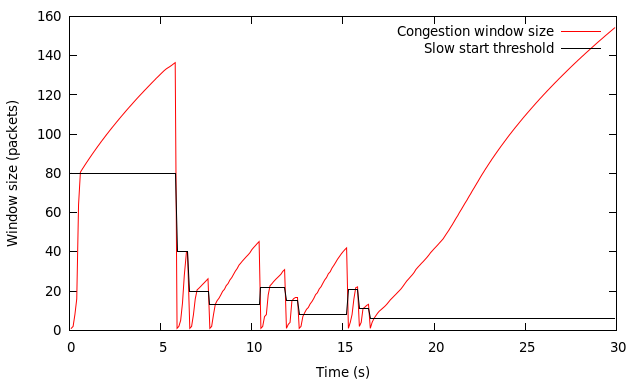
\includegraphics[scale=0.5]{ex2congestionwindow.png}
  \caption{The congestion window sizes and slow start thresholds for the main FTP application running TCP Tahoe.}
 \end{figure}
 
 \item \textbf{Discuss the AIMD principle of TCP. Take one 'sawtooth' pattern in the graph and indicate a few
 reasonable values for the congestion window on the graph. What is the first interval the TCP congestion avoidance
 algorithm is active?} \\
 
 AIMD stands for Additive Increase Multiplicative Decrease. It is the idea where one wants to increase the congestion window
 size by one each round-trip time and, when necessary, decrease the window size multiplicatively. In TCP Tahoe, this
 multiplicative decrease is implemented by cutting the window size to one packet if packet loss occurs. TCP diverges
 from the principle by the use of slow start, where the window size increases exponentially (by always doubling the
 window size) until a pre-defined threshold is reached. After that, it goes back to additive increase. In TCP Tahoe,
 slow start is executed often, while in TCP Reno this only happens when a connection is first established and
 whenever fast recovery fails, which is explained later on in this section. \\
 
 When one plots the behaviour exhibited by a connection that abides by the AIMD principle, it produces a sawtooth pattern.
 There are periods where the congestion window size increases, overshoots the optimal window size, decreases, falls
 below the optimal window size and then increases again. The effect of applying AIMD
 is that the congestion window size converges to the optimal value. Looking at the moment where the first burst begins at 5 seconds in \ref{fig:ex2congestionwindow},
 there is a first drop to a size of one packet. After that, slow start is activated again and the window size increases
 rapidly to 40 packets, after which congestion immediately manifests itself again. The next slow start increases until
 a size of 20, after which additive increase continues for about 600 milliseconds when there is packet loss again.
 After this drop, the intensity of the current burst decreases. This behaviour suggests that a congestion window size
 of 20 would have been a reasonable value during this burst. \\
 
 For the first burst, the congestion avoidance algorithm is active from about 5.76 seconds to 7.95 seconds, whereafter
 additive increase continues unimpeded until after the start of the next burst.
 
 \item \textbf{Change the TCP implementation of the main FTP application into Reno. Plot the congestion window
 and slow start thresholds. Do you spot the differences with the default TCP Tahoe implementation? Why does the
 window sometimes still drop to zero or one?} \\
 
 Figure \ref{fig:ex2congestionwindowreno} shows the behaviour for the TCP Reno implementation. Looking at the congestion drop
 that occurs at approximately 10.6 seconds, it can be seen that both the congestion window size and the slow start threshold
 are set to $max(2, \frac{threshold}{2})$. After that, the window size increases additively. Reno differs in this from
 Tahoe, because Tahoe drops the congestion window size to one packet and then runs a slow start until the new threshold
 is reached. \\
 
 Both Tahoe and Reno take action in order to prevent congestion as well as possible if three duplicate acknowledgements are
 received for the same packet. Reno halves the congestion window. After that it enters fast recovery mode, where it
 resends the lost packet and waits for an acknowledgement for the entire window. If the acknowledgement for
 the resent segment times out, the congestion window size is set to one segment and slow start is activated. This explains
 why the congestion window size is still sometimes set to one.
 
 \begin{figure}[h]
 \label{fig:ex2congestionwindowreno}
  \centering
    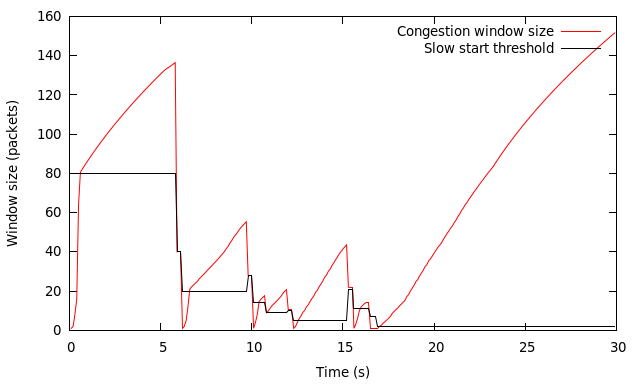
\includegraphics[scale=0.5]{ex2congestionwindowreno.png}
  \caption{The congestion window sizes and slow start thresholds for the main FTP application running TCP Reno.}
 \end{figure}
 
 
\end{enumerate}



\end{document}
